\documentclass[11pt,fleqn]{exam}
\usepackage[utf8]{inputenc}

\usepackage[margin=1in]{geometry}
\usepackage{amsmath,amssymb}
\usepackage{gensymb}
\usepackage{multicol}
\usepackage{float}
\usepackage{graphicx}
\usepackage{units,icomma}
\usepackage[colorlinks,linkcolor=blue,urlcolor=blue]{hyperref}
\usepackage[margin=1.5cm]{caption}

\hyphenation{
  chro-no-ampe-ro-met-ric
  ber-dia-me-ter
  de-ngan
  me-nem-pati
  mic-ro-graphs}

\renewcommand{\figurename}{Gambar.}
\def\equationautorefname{Persamaan}
\newcommand{\class}{OLIMPIADE ASTRONOMI}
\newcommand{\term}{Tingkat Kabupaten/Kota - 2015}
\newcommand{\examnum}{OSK Astronomi 2015}
%\newcommand{\examdate}{11/02/2014}
%\newcommand{\timelimit}{120 Minutes}

\pagestyle{head}
\firstpageheader{}{}{}
\runningheader{\examnum}{}{Halaman \thepage\ dari \numpages}
\runningheadrule


\begin{document}

\noindent
\begin{tabular*}{\textwidth}{l @{\extracolsep{\fill}} r @{\extracolsep{6pt}} l}
\textbf{\class} \\% & \textbf{Name:} & \makebox[2in]{\hrulefill}\\
\textbf{\term}  %&&\\
%\textbf{\examnum} &&\\
%\textbf{\examdate} &&\\
%\textbf{Time Limit: \timelimit} & Teaching Assistant & \makebox[2in]{\hrulefill}
\end{tabular*}\\
\rule[2ex]{\textwidth}{2pt}

\noindent
\begin{tabular}{ll}
Copyright (c) 2015 & Ridlo W. Wibowo (ridlo.w.wibowo@gmail.com)\\
                   & Sulistiyowati (sulis.astro08@gmail.com)
\end{tabular}

\vspace{0.3cm}
\noindent
Solusi ini dibuat tanpa jaminan kesesuaian dengan solusi resmi dari juri olimpiade sains bidang Astronomi. Pengguna boleh menyebarluaskan dan/atau memodifikasi solusi ini dengan mencantumkan sumber asli. Hak cipta soal ada pada Kemendiknas dan dilindungi undang-undang.

\vspace{0.4cm}
\noindent
\rule[2ex]{\textwidth}{1.5pt}

\textbf{Soal Pilihan Berganda}

\begin{questions}
\question Gambar di bawah ini menunjukkan skala sudut deklinasi sebuah teleskop yang dilengkapi skala nonius. 
\begin{figure}[H]
\centering
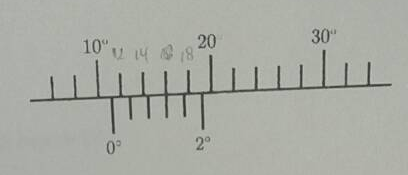
\includegraphics[width=0.4\textwidth]{gambar/nonius.png}
\end{figure}
Berapakah sudut deklinasi yang terukur?
\begin{choices}
\choice $10,04\degree$
\choice $10,30\degree$
\choice $11,30\degree$
\choice $11,20\degree$
\choice $11,40\degree$
\end{choices}

\textit{Jawaban: D}\\
Pembacaan skala nonius:
\begin{enumerate}
\item Lihat nilai skala utama di sebelah kiri nol skala nonius. Dalam soal ini: $10\degree$.
\item Lihat skala nonius yang berimpit dengan skala utama. Dalam soal ini: skala ke-3 dari 5.
\item Sudut bacaan: $10\degree+\frac{3}{5}\times 2\degree=11,20\degree$ ($2\degree$ adalah skala yang diwakili oleh 5 strip skala nonius).\\
\end{enumerate}


\question Misalkan terdapat 28 astronom besar abad ini dan mereka setidaknya menjadi pakar di salah satu bidang: keplanetan, fisika bintang, atau kosmologi.

\noindent \textit{Jumlah astronom yang hanya ahli di bidang keplanetan sama dengan jumlah astronom yang ahli di bidang keplanetan dan fisika bintang. Tidak ada astronom yang hanya ahli fisika bintang atau hanya ahli di bidang kosmologi. Ada enam yang ahli di bidang keplanetan dan kosmologi. Kemudian, jumlah astronom yang ahli di bidang fisika bintang dan kosmologi lima kali lebih banyak dibandingkan jumlah astronom yang ahli di ketiga bidang.}

\noindent Bila jumlah astronom yang ahli di ketiga bidang merupakan bilangan genap dan tidak nol, berapakah jumlah astronom yang hanya ahli di bidang keplanetan?
\begin{choices}
\choice 5
\choice 6
\choice 7
\choice 8
\choice 9
\end{choices}

\textit{Jawaban: A}\\
Pernyataan yang dicetak miring di atas dapat diterjemahkan menjadi bentuk diagram seperti pada gambar berikut.
\begin{figure}[H]
\centering
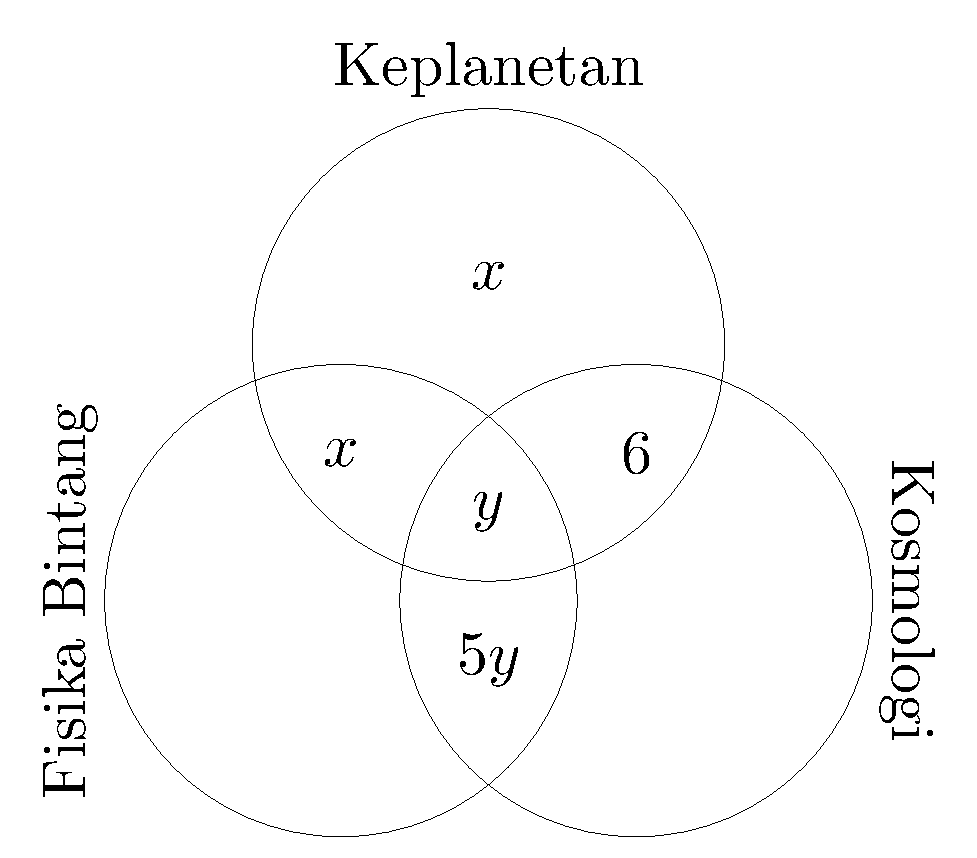
\includegraphics[width=0.4\textwidth]{gambar/himpunan.pdf}
\end{figure}

\noindent Berlaku:
\begin{eqnarray}
x+x+y+5y+6&=&28 \nonumber \\
2x+6y&=&22 \nonumber \\
x+3y&=&11 \label{yeye}
\end{eqnarray}
\noindent disebutkan bahwa $y$ merupakan bilangan genap tidak nol. Hanya ada 1 nilai $y$ yang memenuhi \autoref{yeye}, yakni 2. $y>2$ memberikan $x$ negatif, sehingga tidak mungkin. Jadi, $x=5$.\\

\question Bila $x$ buah teleskop survei dioperasikan selama $x$ jam setiap hari selama $x$ hari, teleskop tersebut dapat menemukan $x$ kandidat planet ekstrasolar. Berapakah jumlah planet yang dideteksi (tidak harus bilangan bulat) oleh sebuah teleskop yang dioperasikan selama $y$ jam setiap hari selama $y$ hari?
\begin{choices}
\choice $\frac{x^3}{y^2}$
\choice $\frac{y^2}{x^2}$
\choice $\frac{x^2}{y^2}$
\choice $\frac{y^3}{x^2}$
\choice $y$
\end{choices}

\textit{Jawaban: B}\\
Laju temuan: $\frac{x}{xxx}=\frac{1}{x^2}$ kandidat per teleskop per jam per hari. Untuk kasus pada soal, jumlah kandidat yang ditemukan: laju penemuan kali jumlah teleskop kali jam operasi kali hari operasi. Jumlah teleskop = 1, karena yang ditanyakan ``oleh sebuah teleskop''. Jumlah kandidat: $\frac{1}{x^2}\times 1\times y\times y=\frac{y^2}{x^2}$.\\


\question Perhatikan gambar di bawah ini.
\begin{figure}[H]
\centering
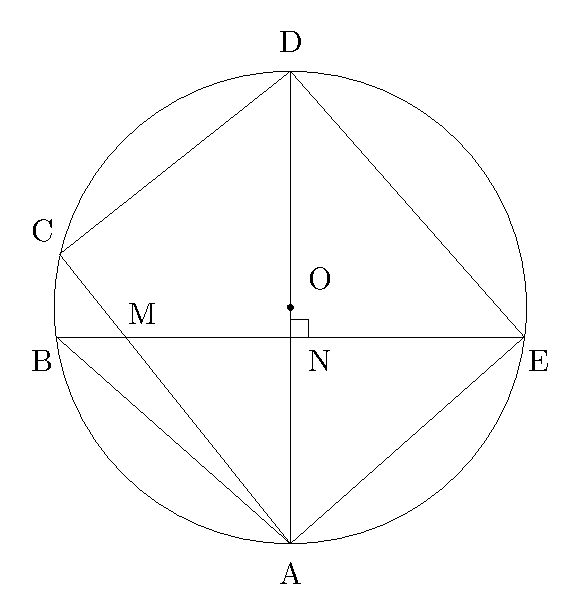
\includegraphics[width=0.3\textwidth]{gambar/lingk-seg4.pdf}
\end{figure}

\noindent Di antara segitiga berikut, manakah yang sebangun dengan $\bigtriangleup AMN$?
\begin{choices}
\choice $\bigtriangleup ACD$
\choice $\bigtriangleup ADE$
\choice $\bigtriangleup ABN$
\choice $\bigtriangleup ABM$
\choice $\bigtriangleup DEN$
\end{choices}

\textit{Jawaban: A}\\
Pada gambar, $\angle ACD$ pasti siku-siku karena sudut tersebut terbentuk di lingkaran, menghadap diameter lingkaran. Dengan demikian, $\angle CDA=\angle NMA$, sehingga $\bigtriangleup ACD$ sebangun dengan $\bigtriangleup AMN$, digambarkan dalam gambar di bawah ini.
\begin{figure}[H]
\centering
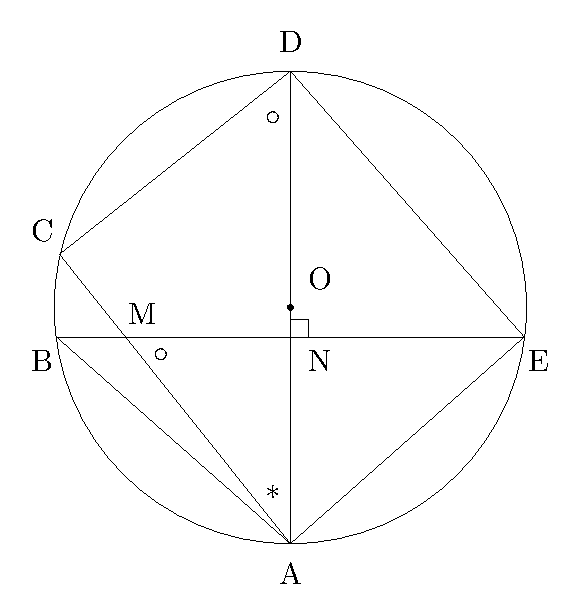
\includegraphics[width=0.3\textwidth]{gambar/lingk-seg4-sol.pdf}
\end{figure}


\question Sebuah planet memiliki massa $M$, volume $V$, serta kerapatan rata-rata $\rho$. Planet hanya terdiri atas inti batuan dengan kerapatan $\frac{3}{2}\rho$ serta mantel es dengan kerapatan $\frac{1}{2}\rho$. Berapakah rasio massa es terhadap massa total planet?
\begin{choices}
\choice 25,0\%
\choice 50,0\%
\choice 66,7\%
\choice 75,0\%
\choice 87,5\%
\end{choices}

\textit{Jawaban: A}\\
Sketsa:
\begin{figure}[H]
\centering
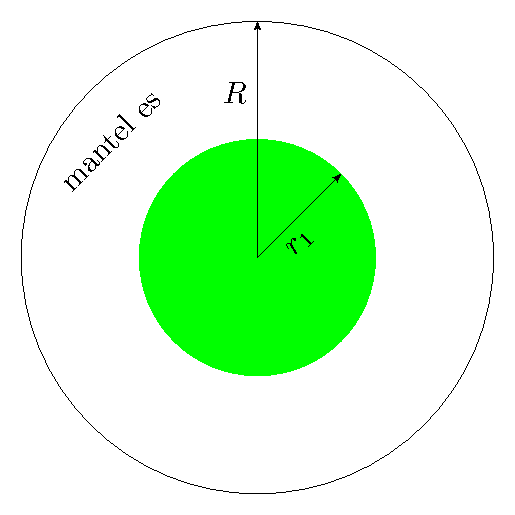
\includegraphics[width=0.3\textwidth]{gambar/planet-es.pdf}
\end{figure}

\noindent Bagian hijau menyatakan inti batuan. Massa total planet merupakan jumlahan antara massa inti $m_b$ dan massa es $m_e$: $M=m_b+m_e$.
\begin{eqnarray}
m_b&=&\rho_b V_b=\frac{3}{2}\rho \frac{4}{3}\pi r_1^3 \nonumber \\
m_e&=&\rho_e V_e=\frac{1}{2}\rho \frac{4}{3}\pi (R^3-r_1^3) \nonumber \\
M&=&\rho V=\rho \frac{4}{3}\pi R^3 \nonumber \\
\frac{m_e}{M}&=&\frac{\frac{1}{2}\rho \frac{4}{3}\pi (R^3-r_1^3)}{\rho \frac{4}{3}\pi R^3} \nonumber \\
 &=& \frac{1}{2}\left(1-\left(\frac{r_1}{R}\right)^3\right) \label{fin}
\end{eqnarray}

\noindent Hitung $\left(\frac{r_1}{R}\right)^3$.
\begin{eqnarray}
M&=&m_b+m_e \nonumber \\
\rho \frac{4}{3}\pi R^3&=&\frac{3}{2}\rho \frac{4}{3}\pi r_1^3+\frac{1}{2}\rho \frac{4}{3}\pi (R^3-r_1^3) \nonumber \\
R^3&=&\frac{3}{2}r_1^3+\frac{1}{2}(R^3-r_1^3) \nonumber \\
1&=&\frac{3}{2}\left(\frac{r_1}{R}\right)^3+\frac{1}{2}\left(1-\left(\frac{r_1}{R}\right)^3\right) \nonumber \\
\frac{1}{2}&=&\left(\frac{r_1}{R}\right)^3
\end{eqnarray}
\noindent Masukkan nilai ini ke dalam persamaan \autoref{fin}, didapat $\frac{m_e}{M}=\frac{1}{4}=25\%$.\\


\question Dalam suatu sistem koordinat kartesian 2 dimensi, lingkaran Bumi dinyatakan dengan persamaan
\begin{equation*}
x(x-4)+y(y-4)=-4
\end{equation*}
\noindent Sebuah partikel neutrino dipancarkan dari titik (4,6) dan mencapai Bumi di titik (2,4). Bila partikel terus bergerak lurus, di titik manakah ia akan keluar menembus Bumi?
\begin{choices}
\choice (0,0)
\choice (1,0)
\choice (2,0)
\choice (0,2)
\choice (0,1)
\end{choices}

\textit{Jawaban: D}\\
Titik-titik yang dilalui garis: ($x_1,y_1$)=(4,6) dan ($x_2,y_2$)=(2,4). Persamaan umum gerak partikel tersebut:
\begin{eqnarray}
y=mx+c
\label{umum}
\end{eqnarray}
\noindent Gradien dan \autoref{umum} menjadi:
\begin{eqnarray}
m&=&\frac{\Delta y}{\Delta x}=\frac{y_2-y_1}{x_2-x_1}=1\\
y&=&x+c
\end{eqnarray}
\noindent Substitusi \autoref{umum} ke titik 1, didapat: $6=4+c$, $c=2$, sehingga persamaan garis yang dilalui partikel menjadi $y=x+2$. Untuk mencari lokasi partikel keluar menembus Bumi, cari perpotongan persamaan garis $y=x+2$ dengan persamaan lingkaran Bumi. Salah satu titik perpotongan seharusnya titik 2 (2,4).
\begin{eqnarray*}
x(x-4)+y(y-4)&=&-4 \\
x(x-4)+(x+2)(x+2-4)&=&-4 \\
x^2-4x+x^2-4&=&-4 \\
2x^2-4x&=&0 \\
x^2-2x&=&0 \\
x(x-2)&=&0 \\
x_1&=&0 \\
x_2&=&2
\end{eqnarray*}
\noindent $x=2$ merupakan titik partikel masuk menembus Bumi, artinya, titik partikel keluar menembus Bumi: $x=0$, $y=x+2=2$, pada titik (0,2).\\


\question Sebuah awan bintang berbentuk bola memiliki radius 100 kali radius Matahari dan memiliki massa 8 kali massa Matahari. Awan tersebut berotasi dengan periode 2000 tahun. Kemudian, awan mengerut hingga radiusnya menjadi 5 kali radius Matahari. Berapakah periode rotasi awan yang telah mengerut?
\begin{choices}
\choice 100 tahun
\choice 50 tahun
\choice 20 tahun
\choice 5 tahun
\choice 1 tahun
\end{choices}

\textit{Jawaban: D}\\
Momentum sudut awan sebelum dan setelah pengerutan kekal. Jika diasumsikan awan seperti bola padat, $I{awan}=\frac{2}{5}m_{awan}r_{awan}^2$. Massa awal ($m_i$) dan massa akhir ($m_f$) sama.
\begin{eqnarray*}
L_i &=& L_f \\
I_i\omega_i &=& I_f\omega_f \\
\frac{2}{5}m_i r_i^2 \frac{2\pi}{P_i}&=&\frac{2}{5}m_f r_f^2 \frac{2\pi}{P_f}\\
P_f&=&\left(\frac{r_f}{r_i}\right)^2 P_i\\
P_f&=&\left(\frac{5R_{\odot}}{100R_{\odot}}\right)^2 2000 \\
P_f&=&5,
\end{eqnarray*}
\noindent dalam satuan tahun.\\


\question Pada tahun 1850-an, John Herschel melakukan pengukuran pancaran energi Matahari yang sampai ke Bumi. Ia memanaskan $10^{-3}$ m\textsuperscript{3} air ($C=4200$ $\text{J}/\text{kg}/\degree \text{C}$) yang awalnya bertemperatur $25\degree$ C menjadi $50\degree$ C. Dengan menggunakan cermin pengumpul seluas 5 m\textsuperscript{2}, ia memerlukan waktu selama 190 detik. Bila kerapatan air dianggap konstan ($\rho=1$ kg/m\textsuperscript{3}), berapakah radiasi Matahari yang diterima Bumi berdasarkan eksperimen Herschel?
\begin{choices}
\choice 560 W/m\textsuperscript{2}
\choice 860 W/m\textsuperscript{2}
\choice 1160 W/m\textsuperscript{2}
\choice 1360 W/m\textsuperscript{2}
\choice 1660 W/m\textsuperscript{2}
\end{choices}

\textit{Jawaban: tidak ada}\\
Kalor yang digunakan untuk memanaskan air: $Q=mC\Delta T= 10^{-3} 4200 (50-25) = 105$ Joule.\\
Daya yang digunakan dalam proses tersebut: $P=\frac{Q}{\Delta t}=\frac{105}{190}=0,55$ Watt.\\
Radiasi Matahari yang diterima Bumi: $\frac{P}{\text{luas cermin}}=\frac{0,55}{5}=0,11$ Watt/m\textsuperscript{2}.\\


\question Gelombang elektromagnetik memiliki rentang spektrum yang amat lebar, dari sinar-$\gamma$ hingga radio. Berapakah perbandingan energi radio 1400 MHz dengan energi sinar-X 100 keV? Diketahui 1 eV=$1,6\times 10^{-19}$ Joule.

\noindent Diketahui konstanta Planck $h=6,63\times 10^{-34}$ Js dan cepat rambat cahaya $3,0\times 10^{8}$ m/s.
\begin{choices}
\choice $10^4 : 1$
\choice $10^1 : 1$
\choice $1 : 10^3$
\choice $1 : 10^7$
\choice $1 : 10^{11}$
\end{choices}

\textit{Jawaban: E}\\ 
Energi pada panjang gelombang radio: $E_r=hf=6,63\times 10^{-34}1400\times 10^6$ JsHz (Hz sama dengan s\textsuperscript{-1}), $E_r=9,28\times 10^{-25}$ Joule.\\
Energi sinar-X: $E_x=100$ keV, $E_x=1,6\times 10^{-14}$\\
Perbandingan: $\frac{E_r}{E_x}=5,8\times 10^{-11}=1,72\times 10^{10}$, jawaban paling mendekati pada orde $1:10^{11}$.\\


\question Orbit $X$ yang mengorbit Matahari diketahui memiliki orbit elips. Bila kecepatan maksimumnya empat kali kecepatan minimumnya, berapa eksentrisitas orbit objek tersebut?
\begin{choices}
\choice 0,0
\choice 0,2
\choice 0,4
\choice 0,6
\choice 0,8
\end{choices}

\textit{Jawaban: D}\\
Pada elips berlaku: $v_r^2=2GM\left(\frac{1}{r}-\frac{1}{2a}\right)$.\\
Kecepatan maksimum $v_p$ didapat ketika jarak minimum (di perihelion) sedangkan kecepatan minimum $v_a$ didapat ketika jarak maksimum (di aphelion).
\begin{eqnarray*}
\frac{v_p^2}{v_a^2}&=&\frac{2GM\left(\frac{1}{r_p}-\frac{1}{2a}\right)}{2GM\left(\frac{1}{r_a}-\frac{1}{2a}\right)} = \frac{\left(\frac{1}{a(1-e)}-\frac{1}{2a}\right)}{\left(\frac{1}{a(1+e)}-\frac{1}{2a}\right)} = \frac{\frac{2-1+e}{2(1-e)}}{\frac{2-1-e}{2(1+e)}} = \frac{(1+e)^2}{(1-e)^2} \\
\frac{v_p}{v_a}&=&\frac{(1+e)}{(1-e)} = 4 \\
4-4e&=&1+e \\
5e&=&3 \\
e&=&0,6\\
\end{eqnarray*}


\question Perhatikan gambar di bawah ini:
\begin{figure}[H]
\centering
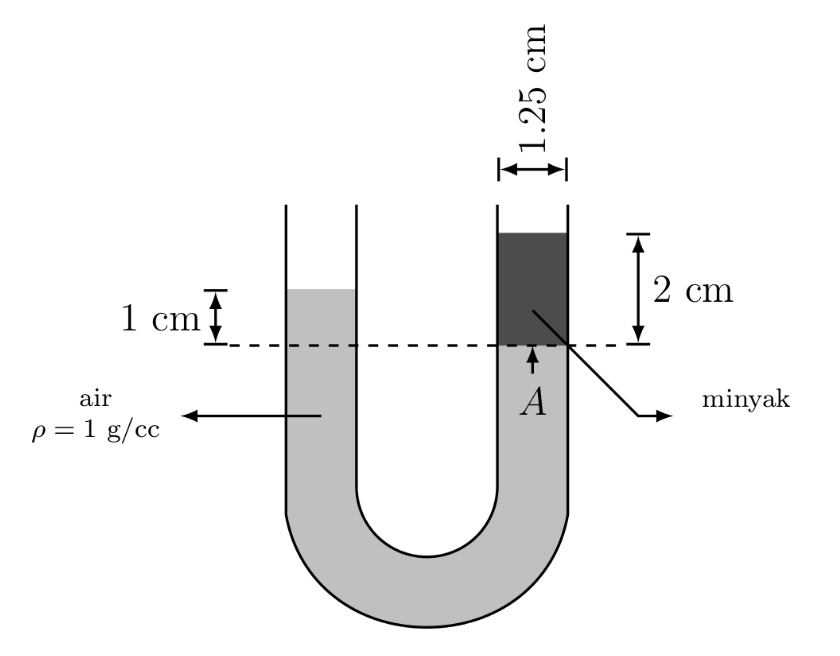
\includegraphics[width=0.4\textwidth]{gambar/tabung.png}
\end{figure}
\noindent Sebuah tabung U berdiameter 1,25 cm diisi dengan air ($\rho=1$ g/cc) dan minyak yang tidak diketahui massa jenisnya. Bila tabung, air, dan minyak tersebut dipindahkan ke Mars yang memiliki gravitasi permukaan 4 m/s\textsuperscript{2} dan tekanan atmosfer $10^4$ Pa, maka ...
\begin{choices}
\choice ketinggian minyak (diukur dari garis batas air-minyak) akan berubah menjadi 0,5 cm.
\choice ketinggian minyak (diukur dari garis batas air-minyak) akan berubah menjadi 0,4 cm.
\choice tekanan hidrostatik di titik A adalah $P_A\approx 4\times 10^4$ Pa.
\choice tekanan hidrostatik di titik A adalah $P_A\approx 1\times 10^4$ Pa.
\choice air akan menguap sebelum pengukuran dapat dilakukan.
\end{choices}

\textit{Jawaban: E} \\
Beda ketinggian antara minyak dan air hanya bergantung pada beda kerapatan mereka. Meskipun lingkungan berubah, karena kerapatan masing-masing tetap, beda ketinggian akan tetap sama.
\begin{eqnarray*}
\rho_{minyak}gh_{minyak}&=&\rho_{air}gh_{air} \\
\rho_{minyak}&=&\frac{h_{air}}{h_{minyak}}\rho_{air} \\
\rho_{minyak}&=&\frac{1}{2}\rho_{air}.
\end{eqnarray*}

\noindent Di Mars, tekanan hidrostatik di A: $P=\rho_{minyak} g_{Mars} h=500\times 4\times 0,02=40$ Pa.\\
Dari hasil ini, opsi A-D tidak mungkin, sehingga opsi yang mungkin adalah E. Selain itu baca kembali berbagai sumber mengenai keberadaan air dalam bentuk cair di Mars. Akan banyak ditemukan penjelasan bahwa air dalam wujud cair akan segera menguap di Mars. 

Berikut diagram fase air, dan terlihat bahwa jika di Bumi dengan berbagai suhu memungkinkan 3 wujud air, yaitu gas, cair, dan padat. Berbeda untuk Mars, tekanan atmosfer yang rendah membuat air tidak mungkin terbentuk dalam wujud cair, berbagai kemungkinan suhu di Mars (garis merah) hanya menghasilkan wujud air sebagai padatan (es di permukaan) atau gas.
\begin{figure}[H]
\centering
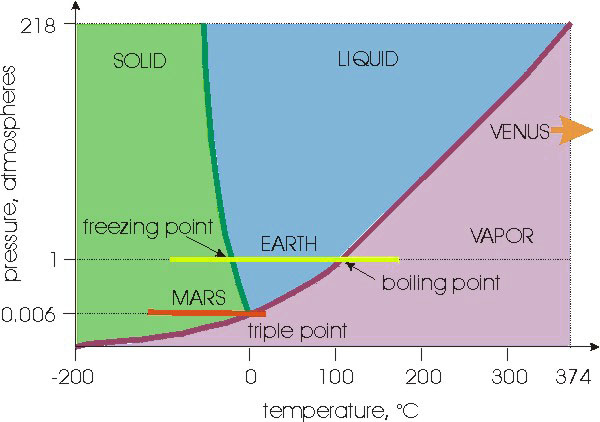
\includegraphics[width=0.5\textwidth]{gambar/mars_phase_diagram.jpg}
\end{figure}
\begin{center}
Source: http://www.iceandclimate.nbi.ku.dk/
\end{center}
\vspace{0.2cm}


\question Benda $A$ bermassa 2 satuan berada di koordinat (-1,2), sedangkan benda $B$ dengan massa 4 satuan berada di koordinat (2,-1). Di manakah posisi pusat massa sistem dua benda tersebut?
\begin{choices}
\choice (0,0)
\choice (4,0)
\choice (6,0)
\choice (1,-4)
\choice (1,-6)
\end{choices}

\textit{Jawaban: tidak ada}\\
Pusat massa sistem: ($x_{pm},y_{pm}$).\\ \\
$x_{pm}=\frac{m_Ax_A+m_Bx_B}{m_A+m_B}=\frac{-2+8}{6}=1$.\\ \\
$y_{pm}=\frac{m_Ay_A+m_By_B}{m_A+m_B}=\frac{4-4}{6}=0$.\\ \\
Koordinat pusat massa: (1,0)\\


\question Terang bintang dinyatakan dalam skala magnitudo ($m$) yang merupakan logaritma dari energinya yang diterima ($E$). Menurut Pogson, $m=-2,5\log E+C$, dengan $C$ menyatakan suatu konstanta.

\noindent Misalkan terdapat dua bintang dengan energi masing-masing $10^2$ dan $10^4$ satuan, sementara bintang pertama memiliki magnitudo +3, berapakah magnitudo bintang kedua?
\begin{choices}
\choice +2 mag
\choice +0 mag
\choice -2 mag
\choice -5 mag
\choice -8 mag
\end{choices}

\textit{Jawaban: C}
\begin{eqnarray*}
m_2-m_1&=&-2,5\log E_2+C - (-2,5\log E_1+C)\\
m_2-m_1&=&-2,5\log \frac{E_2}{E_1} \\
m_2-m_1&=&-2,5\log \frac{10^4}{10^2} \\
m_2-m_1&=&-5\\
m_2&=&-2\\
\end{eqnarray*}


\question Tabel berikut merangkum jumlah bintang dalam rentang magnitudo tertentu yang teramati oleh sebuah teleskop:
\begin{table}[H]
\centering
\begin{tabular}{|c|c|}
\hline
\textbf{Magnitudo} & \textbf{Jumlah} \\
\hline
6,0-8,0 & 10 \\
8,0-10,0 & 23 \\
10,0-12,0 & 45 \\
12,0-14,0 & 30 \\
14,0-16,0 & 11 \\
\hline
\end{tabular}
\end{table}

\noindent Berapakah nilai modus dari distribusi tersebut?
\begin{choices}
\choice 10,0
\choice 10,2
\choice 11,0
\choice 11,2
\choice 12,0
\end{choices}

\textit{Jawaban: D} \\
Pada data berkelompok, nilai modus: $M_o=L+\frac{\Delta f_1}{\Delta f_1+\Delta f_2}C$, $L$ menyatakan tepi bawah kelas modus, $\Delta f_1$ selisih frekuensi kelas modus dengan frekuensi kelas sebelumnya, $\Delta f_2$ selisih frekuensi kelas modus dengan frekuensi kelas setelahnya, $C$ panjang kelas.\\ \\
Untuk soal tersebut: $M_o=10,0+\frac{22}{22+15}3=11,28$. Dalam pilihan jawaban, yang paling mendekati: 11,2.\\


\question Jumlah foton (berpanjang gelombang $\lambda=555$ nm) minimum per detik yang diperlukan untuk menimbulkan rangsangan visual pada mata normal adalah 100 buah. Berapa energi 100 foton tersebut bila dinyatakan dalam watt?

\noindent Diketahui konstanta Planck $h=6,63 \times 10^{-34}$ Js dan cepat rambat cahaya $c=3,00\times 10^8$ m/s.
\begin{choices}
\choice $1,0\times 10^{-17}$ watt
\choice $2,3\times 10^{-17}$ watt
\choice $3,6\times 10^{-17}$ watt
\choice $4,9\times 10^{-17}$ watt
\choice $0,0\times 10^{-17}$ watt
\end{choices}

\textit{Jawaban: C}\\
Energi per satu foton = $\frac{hc}{\lambda} = \frac{6,63 \times 10^{-34} \cdot 3,00\times 10^8}{5,55 \times 10^{-7}} = 3,58 \times 10^{-19}$ joule.\\
Energi 100 foton yang diterima per detik = $3,58 \times 10^{-17}$ watt.\\


\question Seorang insinyur dari LAPAN mengaku menemukan sebuah zat pendingin roket berbahan dasar air. Zat tersebut dilewatkan di antara 3 buah roket yang saling terhubung seperti tampak pada gambar berikut ini.
\begin{figure}[H]
\centering
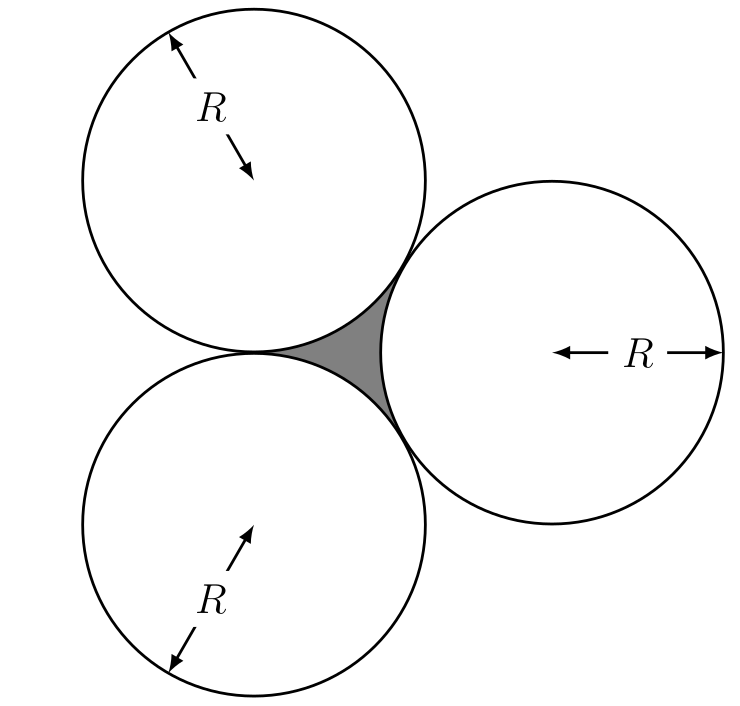
\includegraphics[width=0.3\textwidth]{gambar/pendingin_roket.png}
\end{figure}
\noindent Bila roket memiliki radius $R$ dan tinggi 30 meter, berapakah volume zat pendingin yang dapat dilewatkan pada celah tersebut?
\begin{choices}
\choice $30(\sqrt{3}-\frac{1}{4}\pi)R^2$
\choice $15(\sqrt{\frac{3}{4}}-\frac{1}{2}\pi)R^2$
\choice $30(\sqrt{5}-\frac{1}{3}\pi)R^2$
\choice $60(\sqrt{\frac{3}{4}}-\frac{1}{4}\pi)R^2$
\choice $15(2\sqrt{5}-\frac{1}{4}\pi)R^2$
\end{choices}

\textit{Jawaban: D}\\
Sketsa bantu:
\begin{figure}[H]
\centering
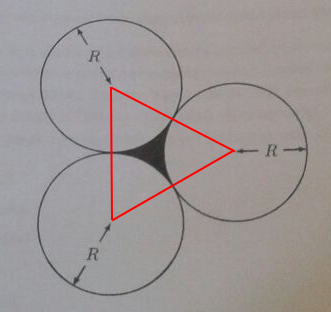
\includegraphics[width=0.3\textwidth]{gambar/pendingin_roket_sol.png}
\end{figure}
Luas segitiga sama sisi = $ \frac{1}{2} \cdot 2R \cdot \sqrt{3} R = \sqrt{3} R^2$.\\
Luas tiga juring = $ 3 \cdot \frac{60\degree}{360\degree} \cdot \pi R^2 = \frac{1}{2} \pi R^2$.\\
Volume celah = $ 30 \left(\sqrt{3} - \frac{1}{2}\pi \right)R^2 = 60 \left(\sqrt{\frac{3}{4}} - \frac{1}{4}\pi \right)R^2$.\\


\question Planet Mars dalam kebudayaan Jawa seringkali disebut sebagai ``bintang'' \textit{Jaka Belek} karena warnanya yang kemerahan. Mengapa planet Mars tampak kemerahan?
\begin{choices}
\choice Karena planet Mars memantulkan cahaya Matahari yang berwarna jingga kemerahan.
\choice Karena atmosfer Mars mengandung gas rumah kaca $\text{CO}_2$ yang menyekat panas.
\choice Karena cahaya planet Mars diserap oleh atmosfer Bumi, maka terlihat kemerahan seperti Matahari saat senja.
\choice Karena planet Mars diselubungi \textit{aerosol} yang menghamburkan cahaya biru.
\choice Karena permukaan Mars diselimuti oksida besi yang berwarna kemerahan.
\end{choices}

\textit{Jawaban: E}\\


\question Planet Venus merupakan planet anggota Tata Surya dengan temperatur global paling tinggi, $T\simeq 700$ K, penyebabnya adalah ...
\begin{choices}
\choice tingginya energi kinetik partikel bermuatan yang dibawa angin Matahari.
\choice pengerutan gravitasi Venus menghasilkan energi termal yang lebih tinggi.
\choice Venus menerima radiasi matahari 90\% lebih banyak dibandingkan Bumi.
\choice konsentrasi karbondioksida di atmosfer Venus amat tinggi, menjebak lebih banyak panas yang diterimanya dari Matahari.
\choice Venus memiliki albedo yang lebih tinggi dibandingkan planet-planet lain.
\end{choices}

\textit{Jawaban: D}\\
Efek rumah kaca (\textit{runaway greenhouse effect}). Energi yang diterima Venus memang lebih besar namun jika hanya itu penyebabnya tidak akan mampu menaikkan suhu hingga 700 K.\\


\question Seorang astronom dari planet San Fierro sedang mengukur diameter sudut dari satelit yang bernama Lupin. Astronom tersebut hanya mengandalkan jengkal tangannya untuk melakukan pengukuran. Diketahui bahwa diameter Lupin adalah 6000 km sedangkan jaraknya dari permukaan San Fierro adalah 15000 km. Berapakah diameter sudut Lupin yang terukur dengan asumsi bahwa satu jengkal tangan setara dengan bentangan sudut $20\degree$?
\begin{choices}
\choice Sekitar 1 jengkal
\choice Sekitar 1/2 jengkal
\choice Sekitar 1/4 jengkal
\choice Tepat 2 jengkal
\choice Tepat 3/2 jengkal
\end{choices}

\textit{Jawaban: A}
\begin{eqnarray*}
\sin{\alpha} &=& \frac{3000}{15000}\\
\sin{\alpha} &=& 0.2\\
\alpha &=& 11.5\degree\\
\delta &=& 2 \alpha = 23\degree
\end{eqnarray*}
Sketsa bantu:
\begin{figure}[H]
\centering
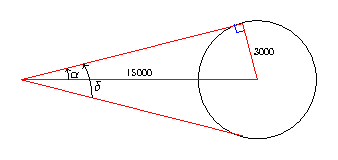
\includegraphics[width=0.5\textwidth]{gambar/diametersudut.pdf}
\end{figure}


\question Diketahui rapat jumlah debu antar bintang sebesar $\rho$ sedangkan luas penampang tiap debu adalah $\sigma$. Maka, jarak rata-rata yang ditempuh setiap debu sebelum bertumbukan dengan debu lain adalah ....
\begin{choices}
\choice $\rho\sigma$
\choice $\frac{\rho}{\sigma}$
\choice $\frac{1}{\rho\sigma}$
\choice $\log \frac{\rho}{\sigma}$
\choice $\left(\frac{\sigma}{\rho}\right)^{1/4}$
\end{choices}

\textit{Jawaban: C}\\
\begin{figure}[H]
\centering
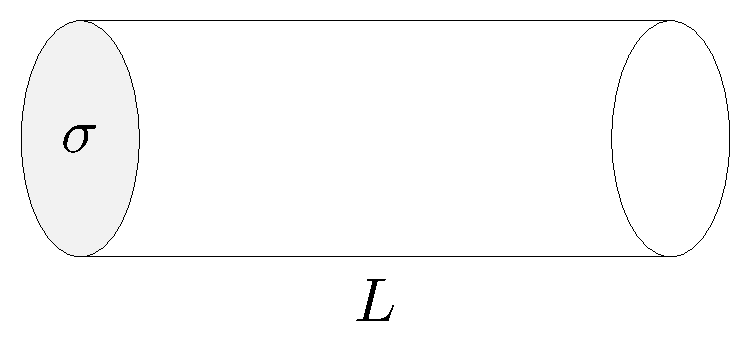
\includegraphics[width=0.3\textwidth]{gambar/mfp.pdf}
\end{figure}
Andaikan luas penampang tumbukan tiap debu adalah $\sigma$, maka sepanjang lintasan $L$ yang ia lalui akan berpeluang bertemu partikel sejumlah $N$. Lintasan tersebut dapat digambarkan sebagai tabung dengan alas $\sigma$ dan panjang $L$. Jumlah partikel yang mungkin ia ``temui'' adalah $N = \rho V = \rho \sigma L $. Sehingga jarak rata-rata tiap tumbukan dapat dihitung:
\begin{eqnarray*}
\text{\textit{mean free path}} = \frac{\text{panjang lintasan}}{\text{jumlah partikel di lintasan}} = \frac{L}{\rho \sigma L} = \frac{1}{\rho \sigma} \\
\end{eqnarray*}


\question Ceres is the largest main-belt asteroid which mainly consists of stone. The mass of this small body is roughly 1/6500 times Earth's mass, while the radius is just 1/13 Earth's radius. How weak does the surface gravity of Ceres pull a falling body, compared to the Earth's gravity?
\begin{choices}
\choice 500 times weaker
\choice 137 times weaker
\choice 38 times weaker
\choice 22 times weaker
\choice 6 times weaker
\end{choices}

\textit{Jawaban: C}\\
$M = \frac{1}{6500} M_{E}$ dan $R = \frac{1}{13} R_{E}$
\begin{eqnarray*}
\frac{g}{g_{E}} &=& \frac{\frac{GM}{R^2}}{\frac{GM_{E}}{R_{E}^2}} = \frac{M}{M_{E}} \left( \frac{R_{E}}{R} \right)^{2}\\
\frac{g}{g_{E}} &=& \frac{1}{6500} 13^{2}\\
g &=& 0.026 g_{E} \quad \text{atau}  \quad \text{38.46 kali lebih kecil.}\\
\end{eqnarray*}


\question There is a terrestrial planet without atmosphere which the maximum surface temperature is mainly governed by three factors: (1) incoming radiation from its star, (2) albedo or reflectance of the planet, and (3) its rotation. Among the following statements, which one is correct?
\begin{choices}
\choice Planet's maximum temperature will be lower if the planet rapidly rotates around its axis.
\choice Planet's maximum temperature will be higher if the planet rapidly rotates around its axis.
\choice If the planet has high reflectivity, then the maximum temperature will be higher.
\choice If the planet has low albedo, then the maximum temperature will be lower.
\choice High stellar radiation melts the ice polar cap and chill the planet.
\end{choices}

\textit{Jawaban: A}\\
Rotasi yang cepat membuat suhu permukaan yang menghadap (siang) dan tidak menghadap bintang (malam) menjadi lebih merata. 

Albedo atau reflektansi merupakan perbandingan energi yang dipantulkan dengan yang diterima, sehingga semakin besar nilainya maka semakin rendah temperatur maksimumnya dan sebaliknya.\\


\textbf{Gunakan petunjuk ini untuk menjawab soal-soal berikut:}\\
A. 1, 2, dan 3 benar\\
B. 1 dan 3 benar\\
C. 2 dan 4 benar\\
D. hanya 4 benar\\
E. semua salah\\

{%
% changing choice items style locally
\renewcommand*\thechoice{\arabic{choice}} 
%
\question Misalkan $a \blacktriangleright b$ menyatakan operasi dua bilangan $a$ dan $b$ yang menghasilkan nilai terbesar antara keduanya, sedangkan $a \blacktriangleleft b$ menghasilkan bilangan terkecil antara keduanya. Berlaku pula hubungan $a \blacktriangleright a = a$ dan $a \blacktriangleleft a = a$.
Di antara pernyataan berikut mana yang benar?
\begin{choices}
\choice $a \blacktriangleright b = b \blacktriangleright a$
\choice $a \blacktriangleright (b \blacktriangleright c) = (a \blacktriangleright b) \blacktriangleright c$
\choice $a \blacktriangleleft (b \blacktriangleright c) = (a \blacktriangleleft b) \blacktriangleright (a \blacktriangleleft c)$
\choice $a \blacktriangleleft (b \blacktriangleright c) = (a \blacktriangleleft b) \blacktriangleright c$
\end{choices}

\textit{Jawaban: A}\\
No 1 dan 2 jelas benar sehingga 3 juga kemungkinan benar.
Cara paling mudah, dicoba untuk nilai $a > b$ dan $c$,  $a <  b$ dan $c$, dan nilai $a$ diantara $b$ dan $c$. :)\\


\question Bila diketahui bahwa vektor $\overrightarrow{A} = 2i + j - k$ dan vektor $\overrightarrow{B} = i -2j + 2k$, maka pernyataan yang benar adalah
\begin{choices}
\choice $\overrightarrow{A} + \overrightarrow{B} = 3i - j + k$
\choice $\overrightarrow{A} \cdot \overrightarrow{B} = 2i - 2j - 2k$
\choice $\overrightarrow{C} = \overrightarrow{A} \times \overrightarrow{B}$ berada di bidang $yz$
\choice $\overrightarrow{A}$ dan $\overrightarrow{B}$ membentuk sudut $< 60^{\circ}$.
\end{choices}

\textit{Jawaban: B}
\begin{eqnarray*}
\overrightarrow{A} \cdot \overrightarrow{B} &=& (2 \cdot 1) + (1 \cdot -2) + (-1 \cdot 2) = 2\\
\Vert A \Vert \Vert B \Vert \cos \theta &=& 2\\
\sqrt{6} \sqrt{9} \cos \theta &=& 2\\
\theta &=& 74.2\degree 
\end{eqnarray*}
\begin{eqnarray*}
\overrightarrow{C} &=& \overrightarrow{A} \times \overrightarrow{B} \\
&=& 
\left|
\begin{matrix}
1 & -1 \\
-2 & 2 
\end{matrix}
\right| i - 
\left| 
\begin{matrix}
2 & -1 \\
1 & 2 
\end{matrix} \right| j +
\left|
\begin{matrix}
2 & 1 \\
1 & -2 
\end{matrix}
\right| k\\
&=& 0 i - 5 j - 5 k \\
&& \text{berada di bidang $yz$}
\end{eqnarray*}


\question On November 14th 2014, Rosetta project operated by European Space Agency has successfully landed its spacecraft on the surface of comet C67/P Churyumov-Gerasimenko. The landing was hard process, but a great achievement because of the following reason, except...
\begin{choices}
\choice The comet exerts a very low gravitational force to the spacecraft.
\choice there are so many debris encircling the comet.
\choice the spacecraft bounced several times before it actually landed.
\choice at that time, the comet was located very far away from Earth, outside the orbit of Neptune.
\end{choices}

\textit{Jawaban: D}\\
Orbit komet berada di dalam orbit Jupiter ketika Rosetta (Philae) mendarat, jadi pernyataan ke-4 salah. Sedikit gas dan debu akan dikeluarkan oleh komet, ``mungkin'' dapat mengganggu misi (misal dapat \href{http://www.esa.int/Our_Activities/Space_Science/Rosetta/Frequently_asked_questions}{menutupi solar panel}). Ingat ada kata \textit{except} di situ sehingga jawabannya D. Sumber: cari berita terkini sains dan astronomi.\\
}%


\textbf{Gunakan petunjuk ini untuk menjawab soal-soal berikut:}\\
A. Pernyataan pertama dan kedua benar serta memiliki hubungan sebab-akibat.\\
B. Pernyataan pertama dan kedua benar, tetapi tidak memiliki hubungan sebab-akibat.\\
C. Pernyataan pertama benar, sedangkan pernyataan kedua salah.\\
D. Pernyataan pertama salah, sedangkan pernyataan kedua benar.\\
E. Kedua pernyataan salah.\\


\question Bumi mengalami gerak presesi seperti gasing yang berputar miring. Gerak tersebut mengubah anggota rasi bintang zodiak yang dilalui Matahari setiap tahunnya.
\begin{center}
sebab
\end{center}
Titik \textit{vernal equinox}, yang menandai perpotongan garis ekuator langit dan ekliptika, bergeser ke arah Timur sedikit demi sedikit.

\textit{Jawaban: E}\\
Presesi mengubah arah sumbu rotasi Bumi, namun tidak mengubah bidang ekliptika, sehingga anggota zodiak akan tetap sama. Titik \textit{vernal equinox} di langit bergeser ke arah Barat.\\


\question Jika orbit Bumi berubah menjadi 7 satuan astronomi (sa), maka 1 \textit{parsec} setara dengan $1,55 \times 10^{14}$ km.
\begin{center}
sebab
\end{center}
Satu \textit{parsec} merupakan jarak bintang ketika Matahari, bintang, dan Bumi membentuk sudut sebesar satu menit busur.

\textit{Jawaban: E}\\
Satu \textit{parsec} = \textit{parallax second} merupakan jarak bintang ketika Matahari, bintang, dan Bumi membentuk sudut sebesar satu ``detik'' busur. Jarak satu \textit{parsec} apabila orbit Bumi 7 sa menjadi $2,16 \times 10^{14}$ km.\\


\question Aurora does not occur everyday.
\begin{center}
because
\end{center}
This phenomenon is caused by bombardment of energetic particles from the active Sun.

\textit{Jawaban: D}\\
Aurora terjadi setiap hari, terjadi karena partikel-partikel bermuatan dari angin Matahari yang dibelokkan oleh medan magnet Bumi sebagian sampai ke atmosfer melalui kutub-kutub magnetnya, semakin jelas ketika aktivitas Matahari meningkat. Terlihat atau tidaknya tergantung banyak faktor, antara lain: lintang pengamat (hanya daerah dekat kutub yang bisa melihat), cerah tidaknya langit, siang malam, musim, polusi cahaya, dan tentunya aktivitas Matahari.\\


\question We can see dark and patchy region with less stars around the constellation of Sagittarius, the direction of galactic center.
\begin{center}
because
\end{center}
Our Milky Way galaxy hosts a super-massive black hole in its center that swallows surrounding gas and stars.

\textit{Jawaban: B}\\
Arah pusat terlihat gelap karena banyak debu yang mengisi ruang antar bintang.\\


\question In March 9th 2016, magnificent total solar eclipse will occur and can be observed in several region in Indonesia.
\begin{center}
because
\end{center}
The umbral shadow will be crossing South Sumatra, Kalimantan, and Halmahera island.

\textit{Jawaban: A}\\
Tunggu saja... tanggal 9 Maret 2016! :)

Sumber: cari info peristiwa astronomi.

\href{http://eclipse.gsfc.nasa.gov/SEgoogle/SEgoogle2001/SE2016Mar09Tgoogle.html}{Link NASA}



\end{questions}

\end{document}
